% !TeX root = ../main.tex

\chapter{Experimental Setup}\label{chapter:experimental-setup}

\section{Experimental Setup}
\label{sec:experimental_setup}

This section documents the hardware configuration, software stack, and test facilities that enabled the experimental evaluation of the aerodynamic surface-enhanced quadrotor. The setup was designed to be fully reproducible, with all control and estimation software running on open frameworks and all data recorded for subsequent analysis.

\subsection{Hardware}

\subsubsection{Airframe and Propulsion}
The experimental platform consists of an X-wing aerodynamic surface-enhanced quadrotor (Fig.~\ref{fig:xwing_platform}) with a total mass of \SI{2.5}{\kilogram} (without batteries: \SI{1.75}{\kilogram}). Each of the four T-MOTOR VELOX~V2808 motors produces a maximum static thrust of approximately \SI{22}{\newton}, resulting in a total available thrust of \SI{88}{\newton} and a thrust-to-weight ratio of 3.59 at nominal \SI{22.2}{\volt} (6S~LiPo). The propulsion system employs HQProp 7×3.5×3 three-blade racing propellers optimized for medium–high efficiency in the forward-flight regime.

The wings feature a NACA~0015 airfoil with a length of \SI{450}{\milli\meter} and a chord of \SI{250}{\milli\meter}. Four identical fixed wings are arranged orthogonally (\SI{90}{\degree} between adjacent wings) and mounted with alternating dihedral and anhedral angles of $\pm\SI{45}{\degree}$. The wings are attached to the central frame using two carbon spars (\SI{10}{\milli\meter} outer diameter) clamped into the core structure, allowing for fast removal. The center frame and motor mounts are 3D-printed from standard PLA, while the wing surfaces are printed from lightweight PLA~Aero. The total projected horizontal area of all wings is approximately $S_\mathrm{t} = 0.318~\si{\meter\squared}$.

Each motor is mounted with a \SI{5}{\degree} tilt to improve yaw authority. The center of gravity is located at the geometric center of the vehicle, aligned with the midpoint between all four motors, and approximately at one quarter of the wing chord length from the leading edge.

\begin{figure}[htbp]
\centering
\begin{minipage}[b]{0.48\textwidth}
    \centering
    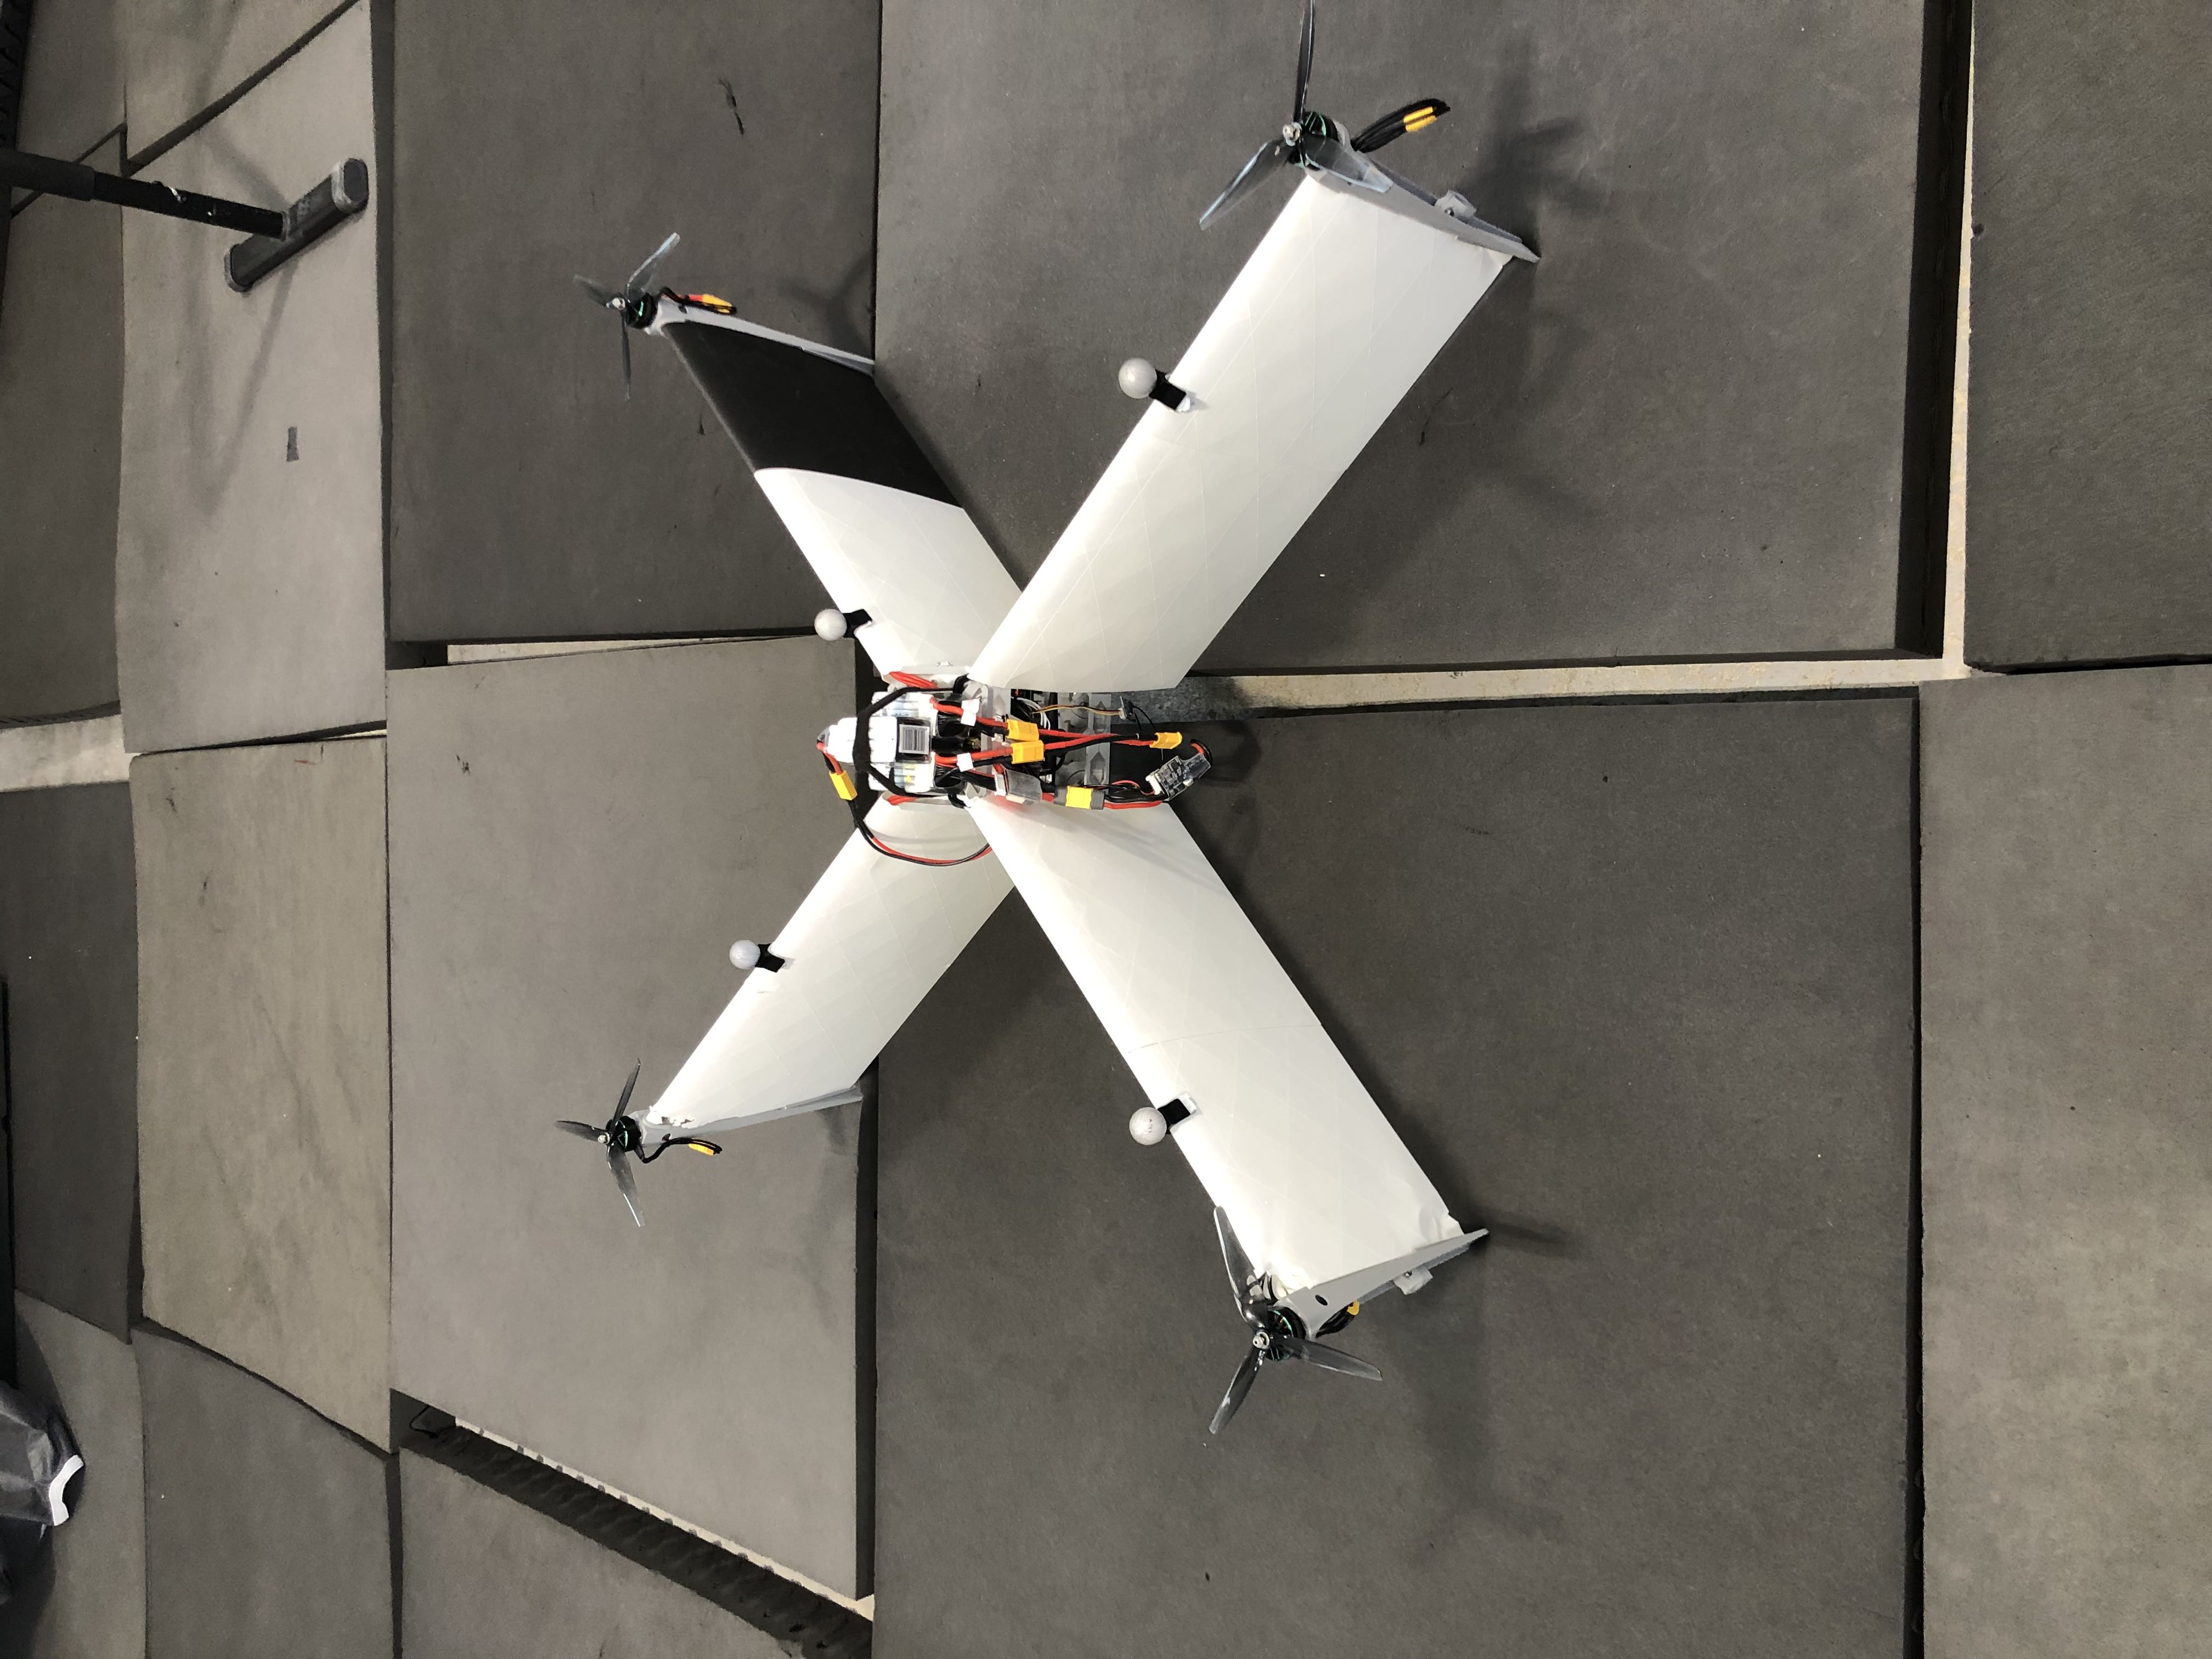
\includegraphics[width=\textwidth,angle=-90]{figures/drone_hover.jpg}
    \caption*{(a) Top view showing X-wing configuration with orthogonal wing arrangement.}
\end{minipage}
\hfill
\begin{minipage}[b]{0.48\textwidth}
    \centering
    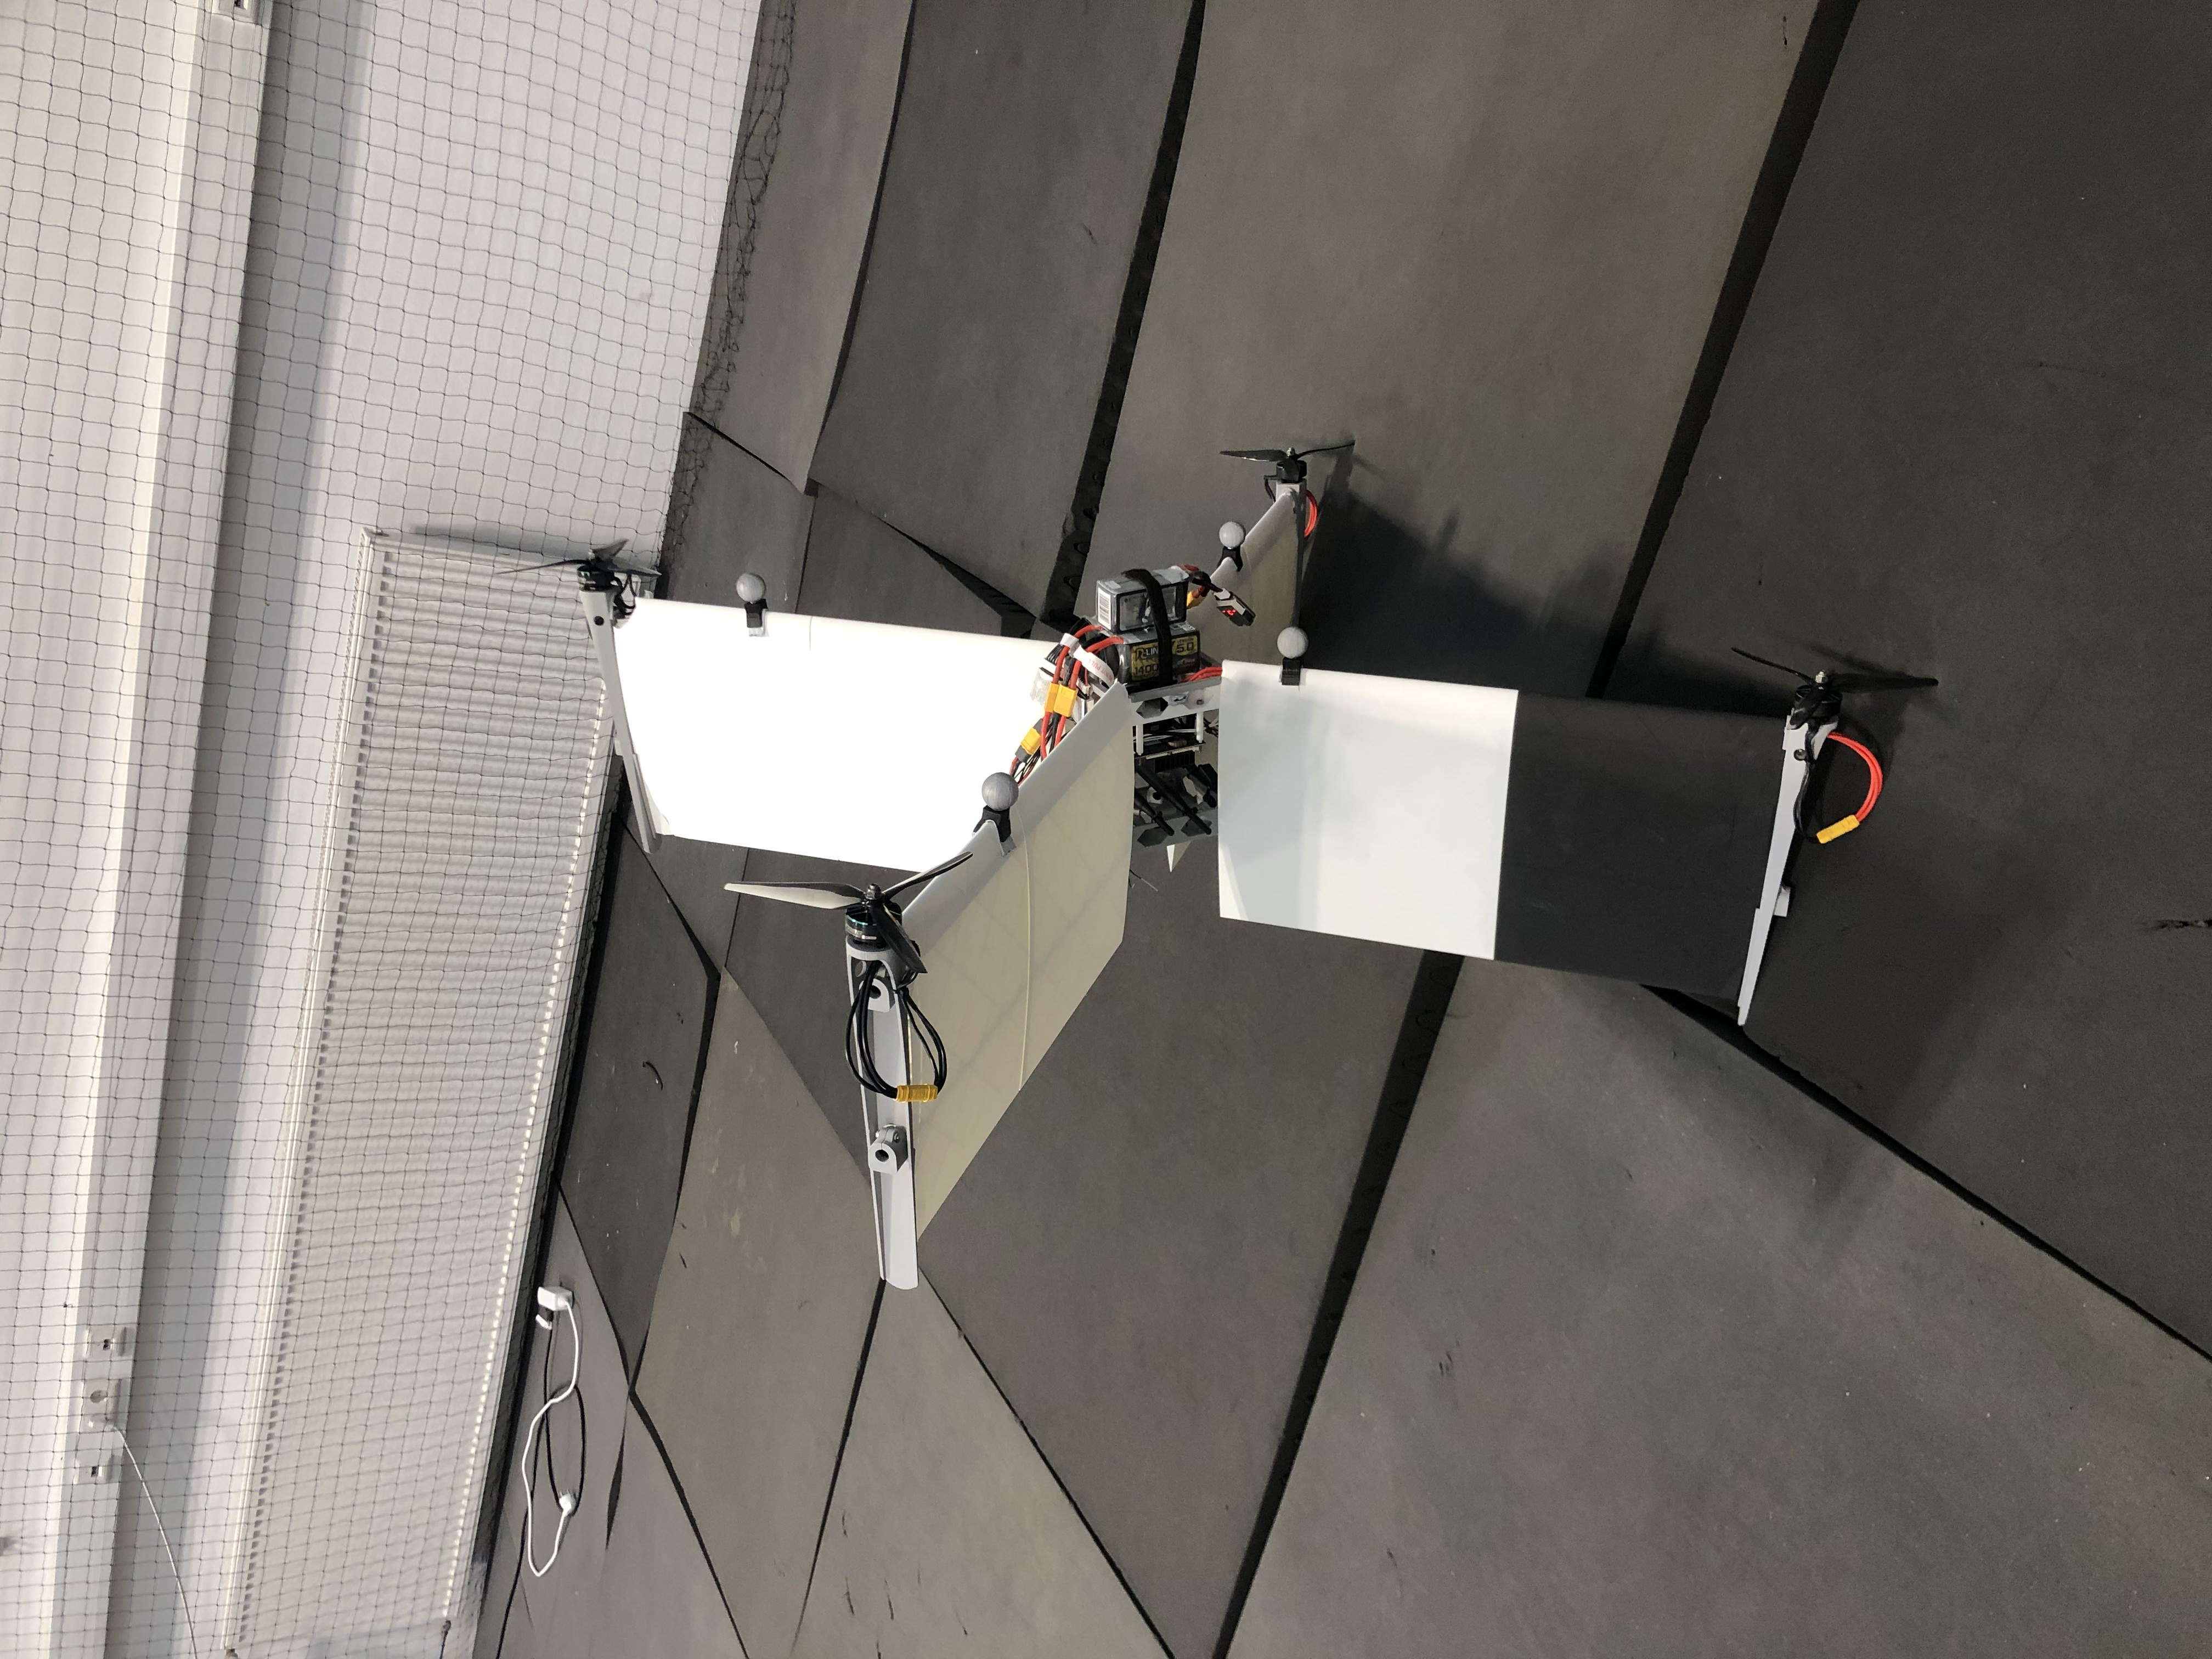
\includegraphics[width=\textwidth,angle=-90]{figures/drone_wing_flight.jpg}
    \caption*{(b) Side view showing forward flight orientation.}
\end{minipage}
\caption{The experimental X-wing aerodynamic surface-enhanced quadrotor platform.}
\label{fig:xwing_platform}
\end{figure}

\subsubsection{Platform Variants}
Two variants of the X-wing platform were used for efficiency experiments. The baseline platform (described above and shown in Fig.~\ref{fig:xwing_platform}) served as the primary testbed for control development and initial efficiency characterization. 

An improved variant with modified aerodynamic characteristics was developed by [Colleague Name]\footnote{[Colleague Full Name], Bachelor thesis, [Lab Name], [Year]. The improved design builds upon the baseline platform and incorporates aerodynamic refinements.} and employed for comparative efficiency measurements. The improved variant features a different airfoil profile and modified dihedral angles optimized for enhanced lift-to-drag performance in forward flight. All other subsystems—propulsion, avionics, mass, and control architecture—remain identical between both platforms, allowing for direct aerodynamic comparison.

Table~\ref{tab:platform_comparison} summarizes the key differences between the two variants.

\begin{table}[h]
\centering
\caption{Comparison of baseline and improved X-wing platform variants.}
\label{tab:platform_comparison}
\small
\begin{tabularx}{\textwidth}{lXX}
\toprule
Parameter & Baseline Platform & Improved Platform \\
\midrule
Airfoil & NACA~0015 & ag25 \\
Dihedral/Anhedral & $\pm\SI{45}{\degree}$ (alternating) & $\pm\SI{20}{\degree}$ (alternating) \\
Wing Length & \SI{450}{\milli\meter} & \SI{500}{\milli\meter} \\
Wing Chord & \SI{250}{\milli\meter} & \SI{230}{\milli\meter} \\
Motor Tilt (Yaw Authority) & $\pm\SI{5}{\degree}$ & $\pm\SI{5}{\degree}$ \\
Total Mass & \SI{2.5}{\kilogram} & \SI{2.2}{\kilogram} \\
Propulsion & T-MOTOR VELOX~V2808 + HQProp 7×3.5×3 & Identical \\
Avionics & Kakute~H7 + Jetson Orin Nano & Identical \\
\bottomrule
\end{tabularx}
\end{table}

\subsubsection{Thrust Characterization and Command Mapping}
To accurately relate motor command inputs to generated thrust, a static thrust characterization was performed for the chosen motor–propeller configuration.  
A single T-MOTOR~VELOX~V2808 motor equipped with an HQProp~7×3.5×3 propeller was mounted on a six-axis force–torque sensor (Rokubi~Mini) using a custom 3D-printed fixture.  
The setup allowed precise measurement of the vertical force while commanding the motor through the same DShot interface used in flight (Fig.~\ref{fig:force_test_stand}).

\begin{figure}[h]
\centering
\begin{tikzpicture}
\node[anchor=south west,inner sep=0] (image) at (0,0) {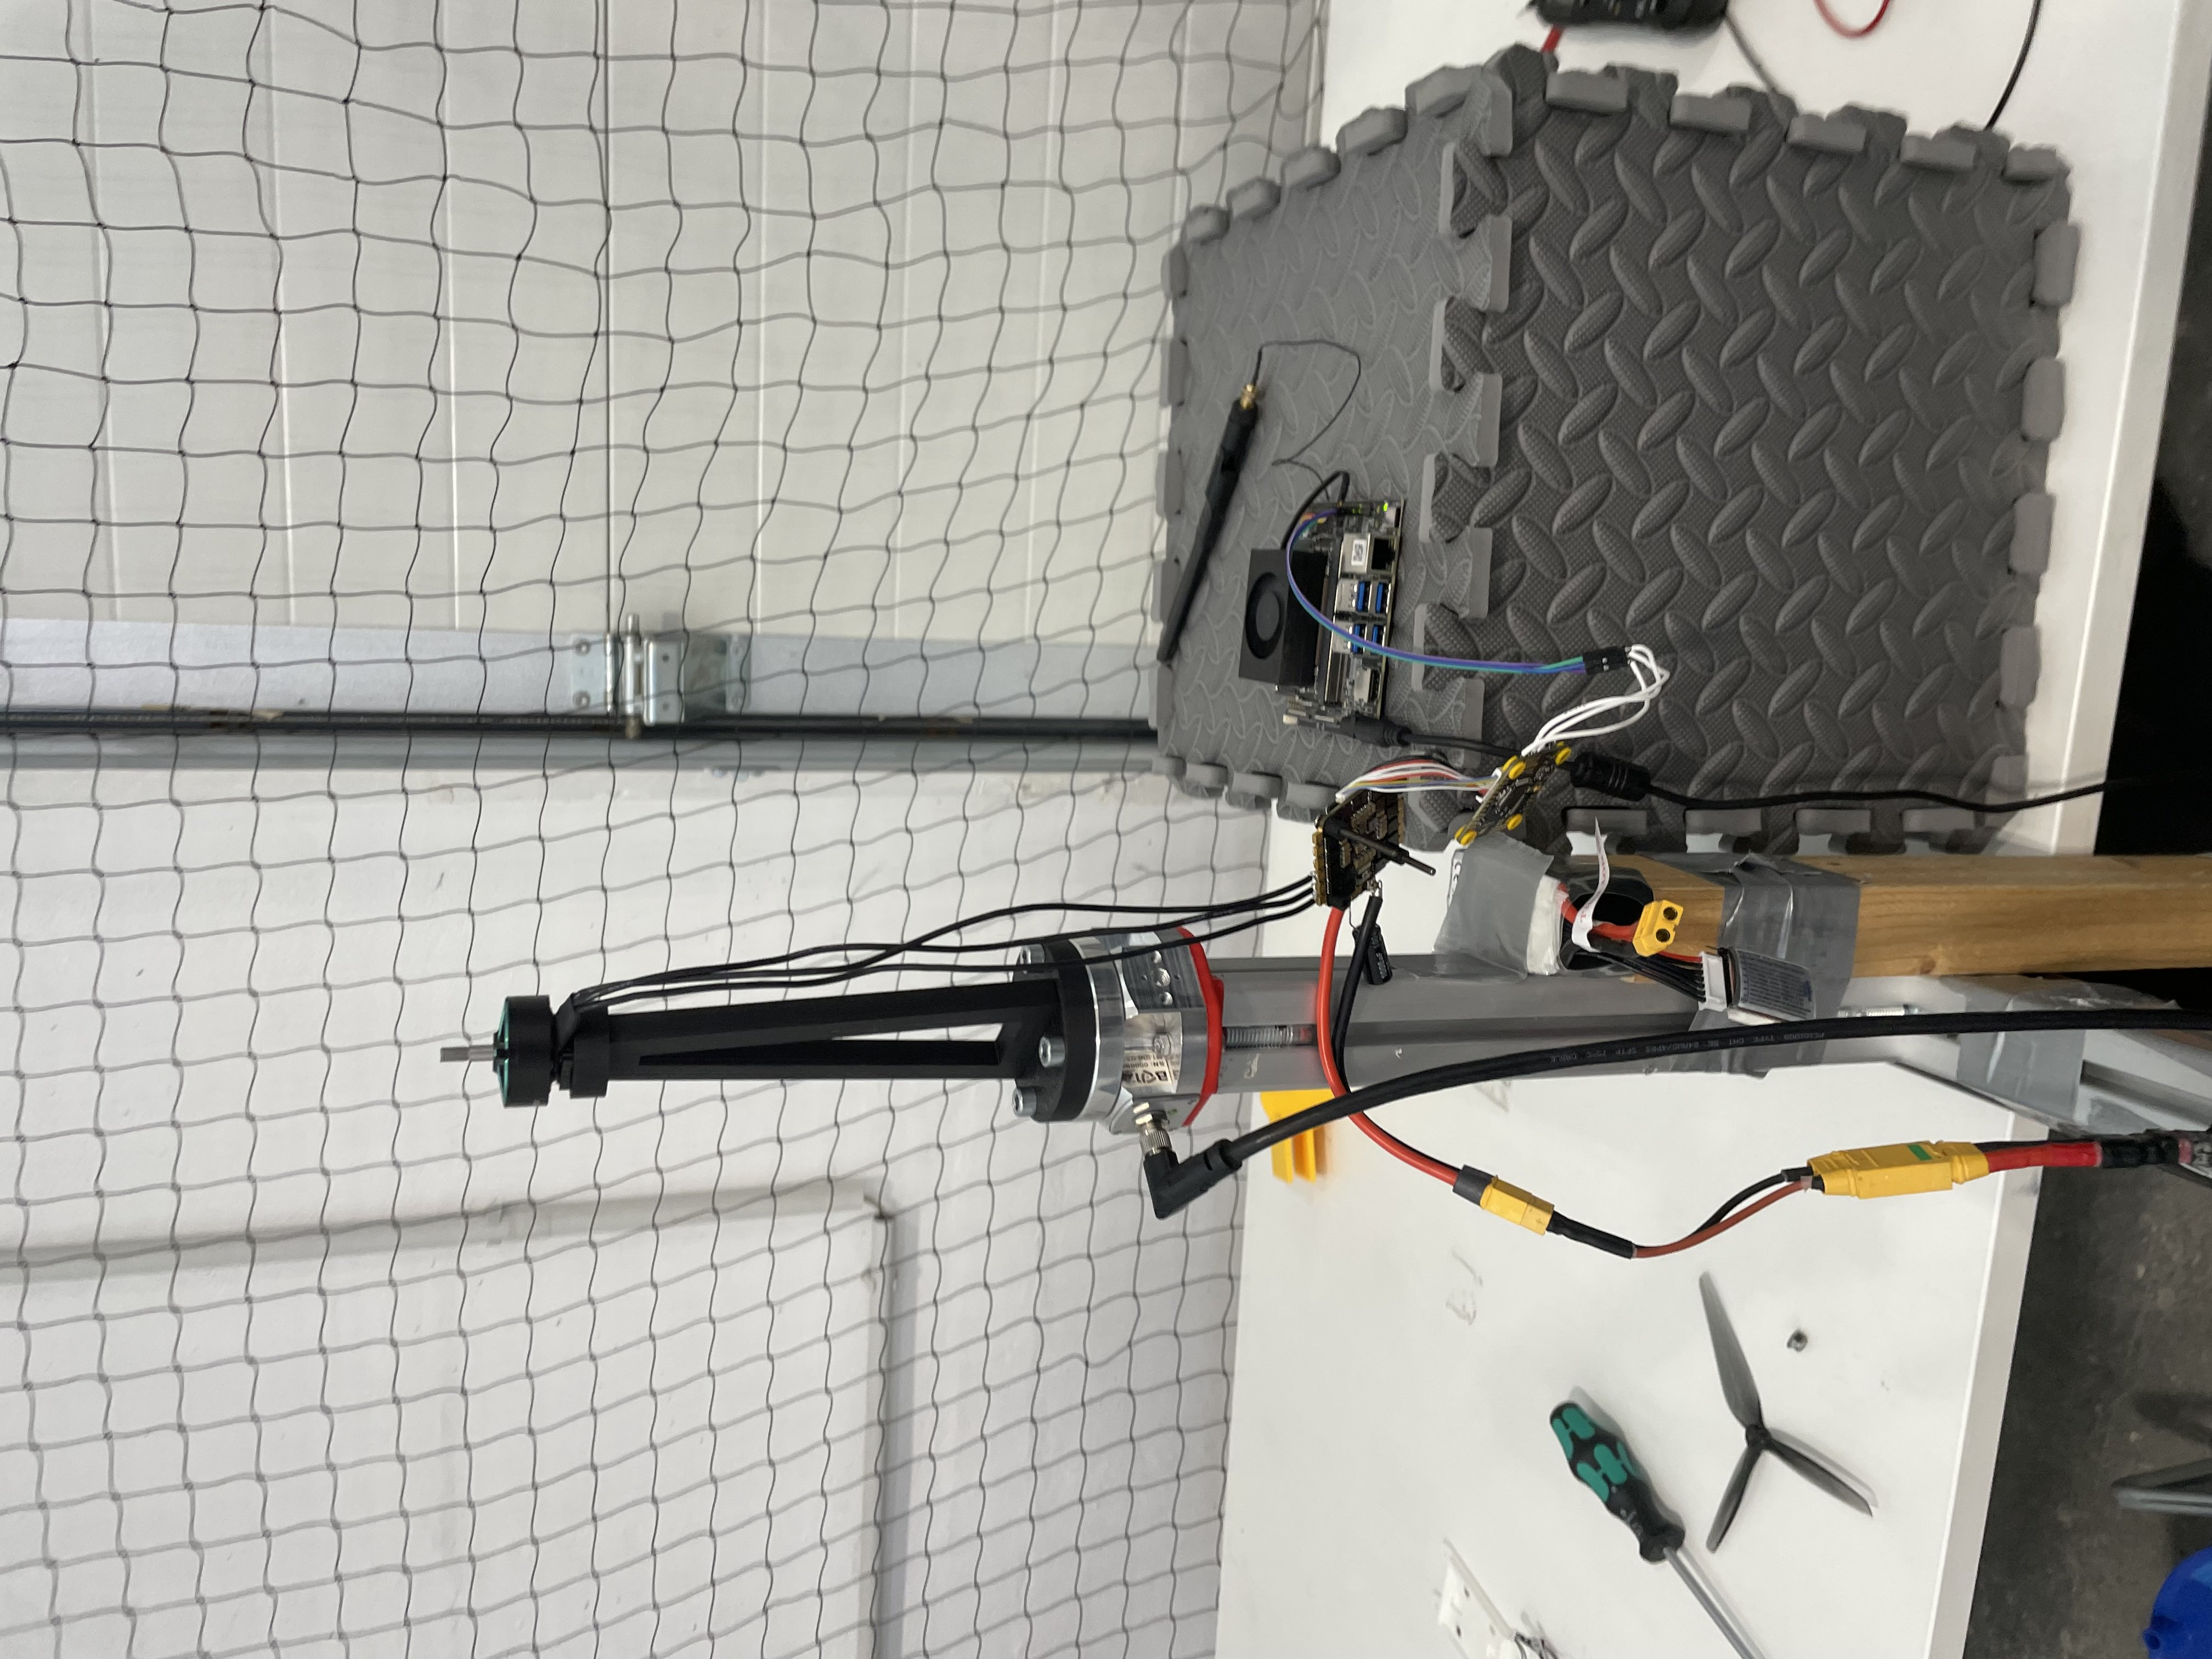
\includegraphics[width=0.85\linewidth,angle=-90]{figures/force_test_stand.jpg}};
\begin{scope}[x={(image.south east)},y={(image.north west)}]
    % Coordinates are relative: (0,0) = bottom-left, (1,1) = top-right
    % Adjust these coordinates to point to the correct components
    
    % Motor at the top
    \draw[->,thick,TUMBlue,line width=4pt] (0.5,0.85) -- (0.4,0.8);
    \node[TUMBlue,font=\normalsize,fill=white,fill opacity=0.85,text opacity=1,inner sep=5pt] at (0.5,0.9) {Motor};
    
    % Force sensor (Rokubi Mini - cylindrical part)
    \draw[->,thick,TUMBlue,line width=4pt] (0.2,0.35) -- (0.3,0.45);
    \node[TUMBlue,font=\normalsize,align=center,fill=white,fill opacity=0.85,text opacity=1,inner sep=5pt] at (0.2,0.3) {Rokubi Mini\\Force Sensor};
    
    % Battery (visible in lower portion)
    \draw[->,thick,TUMBlue,line width=4pt] (0.25,0.15) -- (0.35,0.2);
    \node[TUMBlue,font=\normalsize,fill=white,fill opacity=0.85,text opacity=1,inner sep=5pt] at (0.15,0.15) {Battery};

    % Jetson (visible in lower portion)
    \draw[->,thick,TUMBlue,line width=4pt] (0.75,0.6) -- (0.65,0.5);
    \node[TUMBlue,font=\normalsize,fill=white,fill opacity=0.85,text opacity=1,inner sep=5pt] at (0.75,0.65) {Jetson};

    % FC and ESC (visible in lower portion)
    \draw[->,thick,TUMBlue,line width=4pt] (0.7,0.2) -- (0.55,0.3);
    \node[TUMBlue,font=\normalsize,fill=white,fill opacity=0.85,text opacity=1,inner sep=5pt] at (0.7,0.2) {FC and ESC};
\end{scope}
\end{tikzpicture}
\caption{Static thrust characterization test stand with motor mounted on Rokubi~Mini force–torque sensor.}
\label{fig:force_test_stand}
\end{figure}

Motor command values were swept across the full throttle range in incremental steps, and the resulting thrust was recorded.  
Each command level was averaged over a \SI{2}{\second} window to mitigate transient effects.  
The measurements yielded a nonlinear but monotonic mapping between normalized command input $u \in [0,1]$ and thrust output $T$, which was fitted with a second-order polynomial of the form
\begin{equation}
T(u) = a_2 u^2 + a_1 u + a_0,
\end{equation}
where the coefficients $a_i$ were obtained via least-squares regression.

This empirical mapping was subsequently integrated into the control pipeline to convert desired thrust values from the INDI controller into per-motor DShot commands.  
The calibrated relationship improved the accuracy of total thrust estimation and allowed for energy-based efficiency analysis during flight tests.

\paragraph{Power configuration considerations.}
During the bench tests, one motor was mounted on the force sensor while the remaining four motors stayed on the vehicle and were kept fixed. We observed that the command-to-thrust relationship depends on how many motors are simultaneously powered from the battery due to load-dependent voltage sag and internal resistance effects. In particular, running only a single motor from a single 6S pack produced a slightly different mapping than powering all four motors from the flight-representative configuration with two 6S packs in parallel (6S~2P). Unless stated otherwise, the mapping used for control in flight was calibrated under the latter 6S~2P, four-motor-powered condition, and all subsequent thrust conversions refer to this configuration.

\subsubsection{Avionics and Electrical System}
The avionics stack is based on a \textit{Kakute~H7~v1.5} flight controller paired with a 4-in-1 ESC. Two \SI{1400}{\milli\ampere\hour} 6S~Tattu~R-Line batteries are connected in parallel to power the propulsion and avionics subsystems, resulting in an effective \SI{2800}{\milli\ampere\hour} capacity. The onboard computer, an NVIDIA~Jetson~Orin~Nano~(8\,GB), is powered independently from a \SI{1800}{\milli\ampere\hour} 4S~LiPo battery.

A custom-modified version of \textit{Betaflight} firmware was employed on the flight controller to extract motor RPM and battery voltage data from the DShot interface and stream them over MAVLink. This modification was necessary because the stock Betaflight implementation does not support publishing these telemetry values via MAVLink. The onboard IMU integrated into the Kakute~H7 was used for all experiments; no external IMUs were installed. Vicon markers were arranged asymmetrically to ensure unambiguous pose tracking.

\begin{table}[h]
\centering
\caption{Bill of Materials (BOM) for the experimental platform.}
\label{tab:bom}
\small
\begin{tabularx}{\textwidth}{ll>{\raggedright\arraybackslash}X}
\toprule
Category & Component & Model / Key Specs \\
\midrule
Airframe & Frame & X-wing center frame with carbon wing spars \\
Airframe & Wings & Four fixed wings (length 450\,mm, chord 250\,mm; NACA~0015 airfoil), orthogonal layout ($90^{\circ}$ between adjacent wings); skins: Bambu Lab PLA Aero; spars: 10\,mm OD carbon tubes; total projected horizontal area $S_\mathrm{t}\approx 0.318$\,m$^2$ \\
Propulsion & Motors ($\times$4) & T-MOTOR VELOX~V2808, max~22\,N each \\
Propulsion & Propellers ($\times$4) & HQProp 7\,×\,3.5\,×\,3, 3-blade racing propeller (7", light grey) \\
Avionics & FC+ESC & Kakute~H7~v1.5 Stack (4-in-1~ESC) \\
Power & Battery ($\times$2, parallel) & Tattu~R-Line~V5.0~6S~1400\,mAh~150C, XT60; effective 6S~2800\,mAh (parallel) \\
Companion & Computer & Jetson~Orin~Nano~8\,GB (Ubuntu~20.04) \\
Companion & Power & Tattu~R-Line~V3.0~4S~1800\,mAh~120C, XT60 \\
Motion Capture & Markers & Four 2\,cm markers arranged in an asymmetric constellation \\
\bottomrule
\end{tabularx}
\end{table}

\subsection{Software}

\subsubsection{Architecture and Communication}
The onboard software stack consists of \textit{ROS~1~Noetic} running on the Jetson companion. The geometric controller with inner and outer INDI (Incremental Nonlinear Dynamic Inversion) loops was implemented in ROS and executed on the companion, which sent individual motor speed commands directly to the flight controller over MAVLink via UART. The flight controller, in turn, only relayed the received motor commands to the ESCs while providing IMU, motor RPM, and battery telemetry back to the companion.

A ROS master node was hosted on a ground station computer, while the Jetson ran a ROS node for flight control and data logging. Communication between the two systems was established via Wi-Fi. The ground station handled trajectory loading, arming, and manual control interfaces. All experiment data, including position, velocity, attitude, thrust commands, and battery voltage, were logged in \textit{rosbag} format for offline analysis in Python.

\subsubsection{Estimation and Control}
The state estimation pipeline used the Vicon motion capture system to provide real-time position and attitude feedback to the controller. In some experiments, an onboard Extended Kalman Filter (EKF) fused IMU data for state estimation. The Vicon system and onboard IMU operated in a consistent right-handed coordinate convention (front–left–up), with roll about the $x$-axis, pitch about $y$, and yaw about $z$.

All flight maneuvers, including point-to-point transitions and trajectory tracking, were executed fully autonomously from predefined setpoints. No separate failsafe was implemented for Vicon loss, but trajectories could be manually stopped and the vehicle landed or disarmed from the base station.

\subsection{Facilities}

\subsubsection{Motion Capture Systems}
Two different Vicon systems were employed for data acquisition and feedback.  
The smaller test arena in Munich measured approximately \SI{7}{\meter} × \SI{8}{\meter} and was used primarily for agility experiments, such as \SI{3}{g} circle maneuvers.  
The larger \textit{AIDA Hall} at Reutlingen University provided a volume of about \SI{60}{\meter} × \SI{45}{\meter}, enabling steady forward-flight efficiency trials (see Fig.~\ref{fig:aida_hall}).  
Both systems operated at a sampling rate of \SI{200}{\hertz}.  
Vicon data were used both as ground truth and as feedback for the control loop.

\begin{figure}[h]
\centering
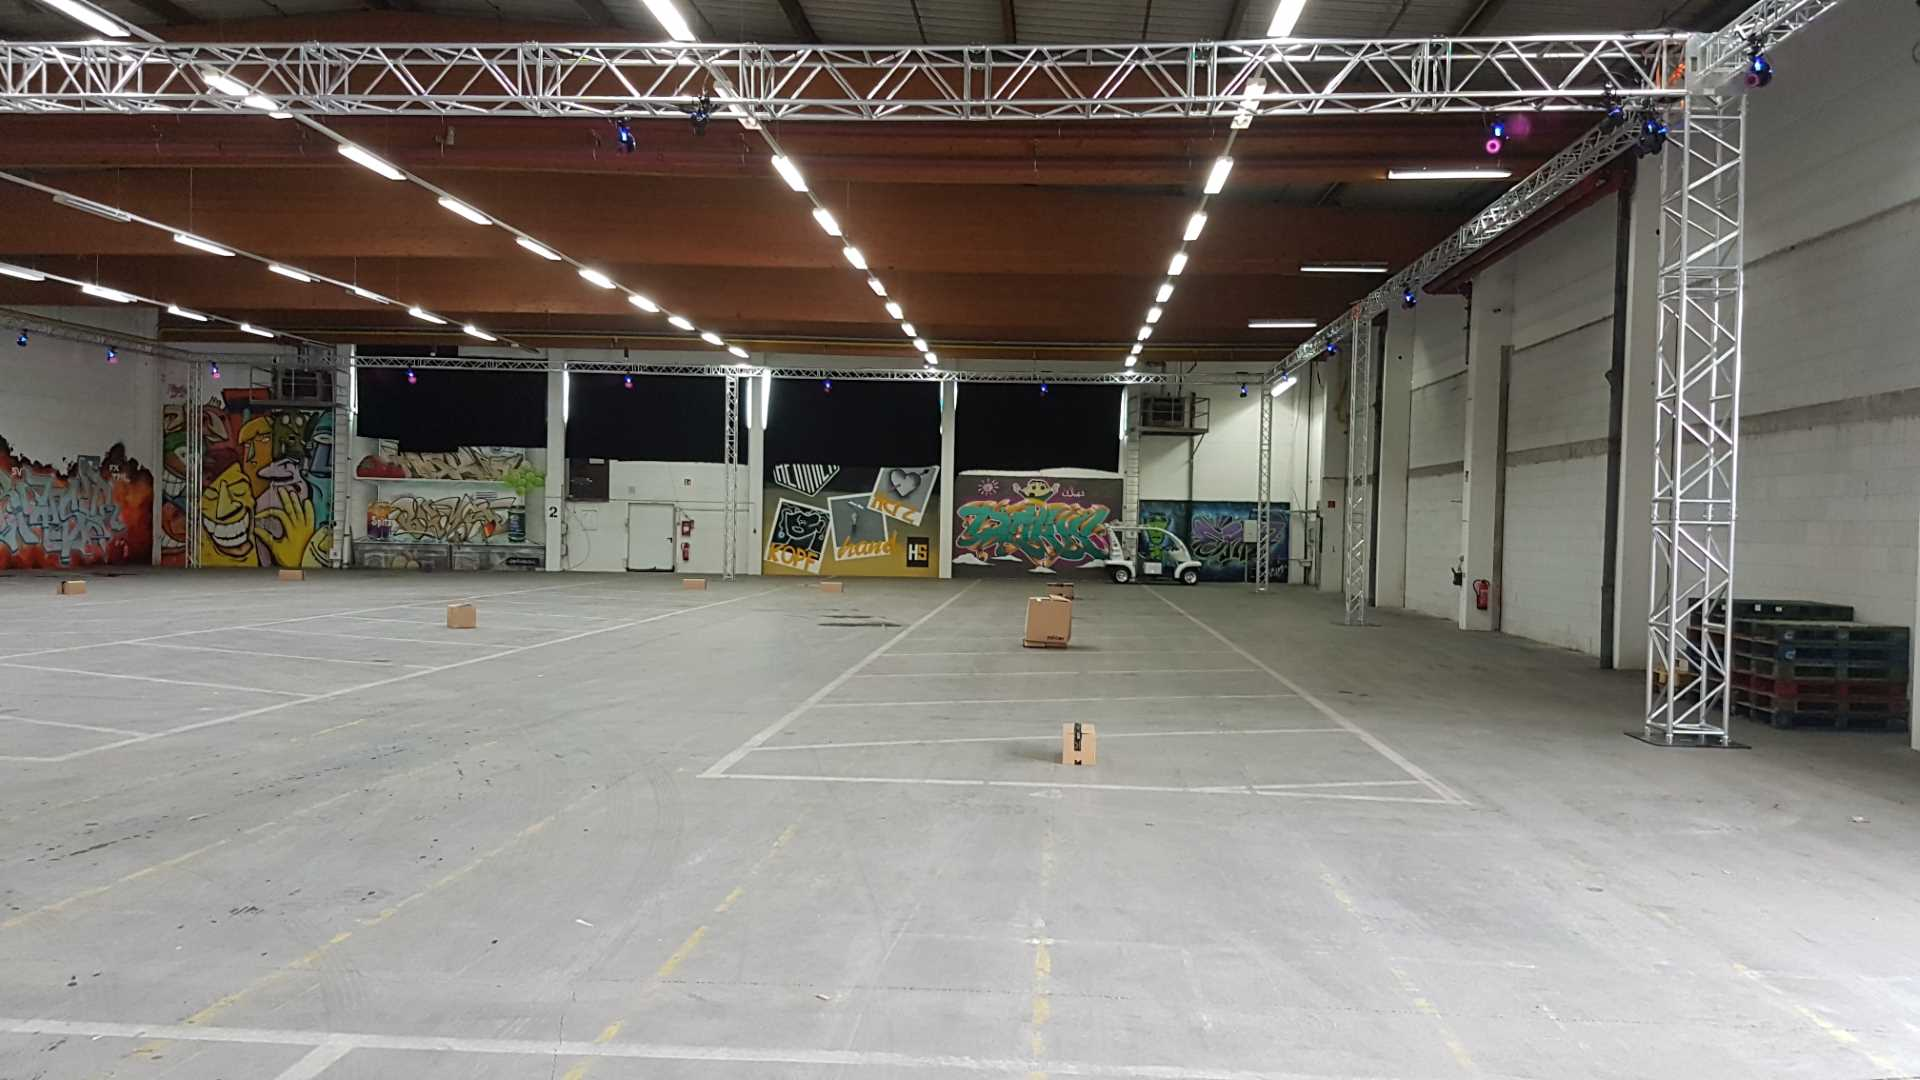
\includegraphics[width=0.85\linewidth]{figures/aida_hall.jpg}
\caption{AIDA Hall test facility used for efficiency trials (image credit: Reutlingen University~\cite{AIDAHallPhoto2024}).}
\label{fig:aida_hall}
\end{figure}

\subsubsection{Test Protocols}
Agility tests were performed in the Munich indoor arena equipped with safety nets and a soft landing surface.  
Efficiency tests were conducted in the AIDA Hall under still-air indoor conditions, with no wind sources or obstacles.  
Energy consumption was estimated from measured voltage, current draw, and propeller rotational speed data.  
Typical flight durations were approximately five minutes per run.

\subsubsection{Documentation}
All experiments were recorded through \textit{rosbag} logs and video footage to facilitate data visualization and reproducibility.  
Post-processing and analysis were conducted in Python, using custom scripts for trajectory evaluation, energy estimation, and control performance comparison.
